\documentclass[12pt]{article}
\usepackage{amsmath, amssymb, enumitem, fancyhdr, graphicx, libertine, nth,
pgfplots, tikz, wasysym, xcolor}
\pgfplotsset{compat=1.11}
\usepackage[margin=1in]{geometry}
\usepackage[libertine]{newtxmath}
\pagestyle{fancy}
\definecolor{solution-color}{HTML}{000080}
\chead{\emph{EC201 -- Problem Set 3 -- Solutions}}

% Define new topic command
\newcommand{\topic}[1]{\medskip\begin{center}\large\textsc{#1}\normalsize
  \end{center}}

% Define question counter:
\newcounter{question}[section]
\newcommand{\question}[1]{\refstepcounter{question}
  \subsubsection*{Question~\thequestion~-- #1}}

% Subquestions are enumerate with letters
\newenvironment{subquestions}{
  \begin{enumerate}[label=(\roman*)]}{\end{enumerate}}

\begin{document}
\topic{Cost Curves}
\question{Cost Curves}
The cost function of a firm is:
\[
  c\left( y \right) = \frac{1}{2}y^2 + 2
\]
\begin{subquestions}
  \item What is the firm's variable cost function $c_v\left( y \right)$?

    \textcolor{solution-color}{
      The variable cost is the portion of the cost function that varies with
      output. These are the terms that include $y$ terms. Here this is just
      $\frac{1}{2}y^2$. So $c_v\left( y \right)=\frac{1}{2}y^2$.
    }
  \item What is the firm's fixed costs?

    \textcolor{solution-color}{
      The fixed cost is the portion of the cost function that doesn't vary with
      output. This is the constant term in the cost function. Here that is 2.
      So $F=2$.
    }
  \item What is the firm's average cost function?
    \textcolor{solution-color}{
      \[
        AC\left( y \right)=\frac{c\left( y
        \right)}{y}=\frac{\frac{1}{2}y^2+2}{y} =
        \frac{\frac{1}{2}y^2}{y} + \frac{2}{y}=
        \frac{y}{2} +
        \frac{2}{y}
      \]
    }
  \item What is the firm's average variable cost function?
    \textcolor{solution-color}{
      \[
        AVC\left( y \right)=\frac{c_v\left( y
        \right)}{y}=\frac{\frac{1}{2}y^2}{y} =
        \frac{1}{2}y
      \]
    }
  \item What is the firm's average fixed cost function?
    \textcolor{solution-color}{
      \[
        AFC\left( y \right)=\frac{F}{y}=\frac{2}{y}
      \]
    }
  \item What is the firm's marginal cost function?
    \textcolor{solution-color}{
      \[
        MC\left( y \right)=\frac{d c\left( y \right)}{dy}=2\cdot
        \frac{1}{2}y^{2-1} + 0 = y
      \]
    }
  \item Verify that the marginal cost curve instersects the average cost curve
    when the average cost curve is at its minimum. That is, first find the
    minimum of $AC\left( y \right)$. Then secondly find $y$ that solves
    $MC\left( y \right)=AC\left( y \right)$.

    \textcolor{solution-color}{
      The minimum of $AC\left( y \right)$ happens when its derivative equals
      zero:
      \[
        \frac{d\left( AC\left( y \right)
        \right)}{dy}=\frac{1}{2}-\frac{2}{y^2}
      \]
      Finding the $y$ where this equals zero:
      \[
        \frac{1}{2}-\frac{2}{y^2}=0\;\;\;\; \Longleftrightarrow \;\;\;\;
        \frac{1}{2}=\frac{2}{y^2}\;\;\;\; \Longleftrightarrow \;\;\;\;
        y^2=4\;\;\;\; \Longleftrightarrow \;\;\;\;
        y = 2
      \]
      Therefore $AC\left( y \right)$ is at its minimum when $y=2$\footnote{
        \textcolor{solution-color}{Note that normally $y^2=4$ implies $y=\pm 2$
      but since output is necessarily positive, we ignore the negative
  solution.}}.
      If we set $MC\left( y \right)=AC\left( y \right)$ we get:
      \[
        y=\frac{y}{2}+\frac{2}{y} \;\;\;\; \Longleftrightarrow \;\;\;\;
        \frac{y}{2}=\frac{2}{y} \;\;\;\; \Longleftrightarrow \;\;\;\;
        y^2=4 \;\;\;\; \Longleftrightarrow \;\;\;\;
        y=2
      \]
      This confirms that $MC\left( y \right)$ and $AC\left( y \right)$
      intersect at the minimum point of $AC\left( y \right)$ in this case.
    }
  \item Sketch the marginal cost, average cost and average variable cost
    function on a graph. Label the intersections of the curves with
    their values on the axes.

    \textcolor{solution-color}{
      The minimum of $AC\left( y \right)$ happens at $\left( 2,2 \right)$ and
      the minimum of $AVC\left( y \right)$ happens at $\left( 0,0 \right)$.
      \begin{center}
        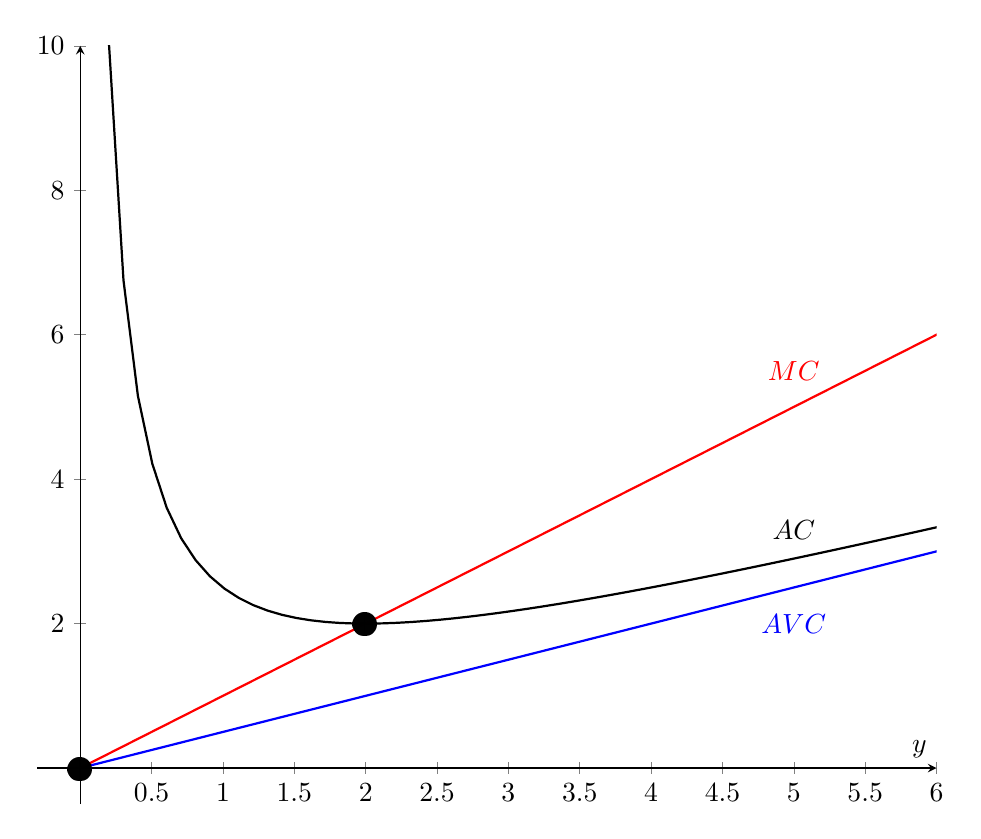
\begin{tikzpicture}[baseline]
          \begin{axis}[xmax=6,xmin=-.3,
                       ymin=-.5,ymax=10,
                       axis lines=middle,
                       width=13cm,
                       xlabel=$y$]
            \addplot[thick, samples=100][domain=0:10] {x/2 + 2/x};
            \addplot[thick, blue, samples=100][domain=0:10] {x/2};
            \addplot[thick, red, samples=100][domain=0:10] {x};
            \draw (5, 3.3) node {$AC$};
            \draw[blue] (5, 2) node {$AVC$};
            \draw[red] (5, 5.5) node {$MC$};
            \draw (2, 1.95) node{\Huge \textbullet};
            \draw (0,-0.05) node{\Huge \textbullet};
          \end{axis}
        \end{tikzpicture}
      \end{center}
    }
\end{subquestions}

\newpage
\topic{Firm Supply}
\question{Short-Run and Long-Run Supply}
Consider the following marginal cost curve ($MC$), average cost curve ($AC$)
and average variable cost curve ($AVC$).
\begin{center}
  \begin{tikzpicture}[baseline]
    \begin{axis}[ticks=none,
                 xmax=10,xmin=-2,
                 ymin=-15,ymax=100,
                 axis lines=middle,
                 width=13cm,
               xlabel=$y$,ylabel=\hspace{-8mm}$\$$]
      \addplot[thick, samples=100][domain=0:10] {15/x + 50-8*x+x^2};
      \addplot[thick, blue, samples=100][domain=0:10] {50-8*x+x^2};
      \addplot[thick, red, samples=100][domain=0:10] {50-16*x+3*x^2};
      \addplot[dashed] coordinates {(0,37.569)(4.389,37.568)};
      \addplot[dashed, blue] coordinates {(0,34)(4,34)};
      \addplot[dashed, red] coordinates {(0,28.666666)(2.6667,28.666666)};
      \draw (0, 37.569) node [left] {$a$};
      \draw[blue] (0, 34) node [left] {$b$};
      \draw[red] (0, 28.66666) node [left] {$c$};
      \addplot[dashed] coordinates {(4.389,0)(4.389,37.568)};
      \addplot[dashed, blue] coordinates {(4,0)(4,34)};
      \addplot[dashed, red] coordinates {(2.66667,0)(2.6667,28.666666)};
      \draw (4.389, -5) node {$f$};
      \draw[blue] (4, -5) node {$e$};
      \draw[red] (2.666667, -5) node {$d$};
      \draw (8, 60) node {$AC$};
      \draw[blue] (9, 50) node {$AVC$};
      \draw[red] (7.5, 80) node {$MC$};
    \end{axis}
  \end{tikzpicture}
\end{center}
The firm is in the \textbf{short run}:
\begin{subquestions}
  \item If $p=a$, how much will the firm produce (in terms of $d$, $e$ and $f$)?

    \textcolor{solution-color}{
      The firm produces the output where $p=MC\left( y \right)$. Thus the firm
      will produce $f$ units.
    }
  \item If $p=a$, what will the firm's profit be (in terms of $a$, $b$, $c$,
    $d$, $e$ and $f$)?

    \textcolor{solution-color}{
      The firm's profit is $\left[ p-AC\left( y \right) \right]y$. Since
      $p=AC\left( y \right)$ the firm will make a zero profit.
    }
  \item If $p=b$, how much will the firm produce (in terms of $d$, $e$ and $f$)?

    \textcolor{solution-color}{
      The firm produces the output where $p=MC\left( y \right)$. Thus the firm
      will produce $e$ units. Here $p=AVC\left( y \right)$ so the firm is
      actually indifferent between temporarily shutting down and producing $e$.
    }
  \item If $p=b$, will the firm be making a profit or a loss?

    \textcolor{solution-color}{
      Here $p<AC\left( y \right)$ so the firm will be making a loss.
    }
  \item If $p=c$, how much will the firm produce (in terms of $d$, $e$ and $f$)?

    \textcolor{solution-color}{
      The firm will temporarily shut down if the price is less than average
      variable cost. This is the case here so the firm  will produce 0 units of
      output.
    }
\end{subquestions}
Now the firm is in the \textbf{long run}:
\begin{subquestions}
  \setcounter{enumi}{5}
  \item If $p<a$, what will the firm do and why?

    \textcolor{solution-color}{
      The firm will be making a loss if $p<a$ and would therefore exit the
      industry in the long run.
    }
\end{subquestions}


\topic{Industry Supply}
\question{Industry Supply}
Consider a competitive industry where every firm has the same cost function
$c\left( y \right)=\frac{1}{2}y^2+1$. The market demand function is
$D\left( p \right) = 220 - 10p$.
\begin{subquestions}
  \item What is the supply function $S_i\left( p \right)$ for an individual
    firm in the industry? Hint: use the firm's optimality condition,
    $p=MC\left( y \right)$.

    \textcolor{solution-color}{
      The marginal cost curve for the firm is $c^\prime\left( y \right)=y$.
      Using $p=MC\left( y \right)$ we get $p=y$. The supply function for one
      firm is then $S_i\left( p \right)=p$.
    }
  \item If there are 100 firms in the industry, what will the industry supply
    curve, $S\left( p \right)$, be?

    \textcolor{solution-color}{
      The industry supply curve just adds up all the individual supply curves.
      This is:
      \[
        S\left( p \right)=S_1\left( p \right)+S_2\left( p
        \right)+\dots+S_{100}\left( p \right) = p + p + \dots + p= 100p
      \]
    }
  \item What will the (short-run) equilibrium price be?

    \textcolor{solution-color}{
      The equilibrium price comes from setting supply equal to demand:
      \[
        S\left( p \right)=D\left( p \right) \;\;\;\Longleftrightarrow \;\;\;
        100p=220-10p \;\;\;\Longleftrightarrow \;\;\;
        110p=220 \;\;\;\Longleftrightarrow \;\;\;
        p=2
      \]
    }
  \item How many units does the industry as a whole produce?

    \textcolor{solution-color}{
      Using $p=2$ in the industry supply function:
      \[
        S\left( p \right)=100p = 100\times2=200
      \]
      The industry as a whole produces 200 units.
    }

  \item How many units does a single firm produce?

    \textcolor{solution-color}{
      Each firm produces output according to their supply function $S_i\left( p
      \right)=p=2$. The 100 firms share the 200 units of output equally and
      produce 2 units.
    }
  \item What profit does each firm make?

    \textcolor{solution-color}{
      The profit for each firm:
      \[
        py- \frac{1}{2}y^2 - 1 = 2\times 2 - \frac{1}{2}\times2^2 - 1 = 1
      \]
      The firms are making profits of 1.
    }
  \item Will any firms want to enter or exit this industry in the long run?

    \textcolor{solution-color}{
      In the long run firms will want to enter this industry since they are
      making profits. Eventually, after enough firms enter. The price will fall
      until they break even
    }
\end{subquestions}

\topic{Equilibrium}
\question{Taxation}
The demand and supply functions for a particular good
in the market are given by:
\[
  D\left( p \right) = 12 - 2p
\]
\[
  S\left( p \right) = 2 + 3p
\]
\begin{subquestions}
  \item Find the equilibrium price and quantity.

    \textcolor{solution-color}{
      To find the equilibrium price, $p^\star$, we set $D\left( p^\star
      \right)=S\left( p^\star \right)$:
    \[
      12-2p^\star=2+3p^\star \;\;\; \Longleftrightarrow \;\;\;
      12-2=2p^\star+3p^\star \;\;\; \Longleftrightarrow \;\;\;
      10=5p^\star \;\;\; \Longleftrightarrow \;\;\;
      p^\star=\frac{10}{5} \;\;\; \Longleftrightarrow \;\;\;
      p^\star=2
    \]
    The quantity can be found by using $p^\star$ in either $S\left( p
    \right)$ or $D\left( p \right)$. Using demand:
    \[
      q^\star = 12 - 2\times 2=8
    \]
    Using supply:
    \[
      q^\star = 2 + 3\times 2=8
    \]
    }
\end{subquestions}
Now the government imposes a per-unit tax (a quantity tax) of 1 on the good.
\begin{subquestions}
  \setcounter{enumi}{1}
  \item Find the price the buyers pay, the price sellers receive and the new
    equilibrium quantity.

    \textcolor{solution-color}{
      Now $P_D=P_S+t$. We can replace $p$ in the demand function with $P_S+t$
      and then set demand equal to supply:
      \begin{align*}
        12 - 2\left( P_S+t \right) &= 2+ 3P_S \\
        12 - 2P_S -2t &= 2 + 3P_S \\
        10  -2t &=  5P_S \\
        5P_S &= 10 - 2t \\
        P_S &= 2 - \frac{2}{5}t \\
        P_S &= 2 - \frac{2}{5}\\
        P_S &= 1.6
      \end{align*}
      Using $P_D=P_S+t$ we can find the price buyers pay:
      \[
        P_D=2 - \frac{2}{5}t + t = 2 +\frac{3}{5}t = 2.6
      \]
      The price increased for buyers by $\frac{3}{5}t=60\cent$ and the price
      decreased for sellers by $\frac{2}{5}t=40\cent$.
    }

    \textcolor{solution-color}{
      The new equilibrium quantity can be found using either the inverse demand
      or supply function. Using demand:
      \[
        q^\star = 12 - 2P_D = 12 - 2 \times 2.6 = 12 - 5.2 = 6.8
      \]
      Using supply:
      \[
        q^\star = 2 + 3P_S = 2 + 3 \times 1.6 = 2 + 4.8 = 6.8
      \]
      The tax decreased the equilibrium quantity by 1.2 units.
    }
  \item What portion of the tax do consumers pay and what portion of the tax do
    sellers pay?

    \textcolor{solution-color}{
      Since the price increased by $\frac{3}{5}$ of the tax for consumers, they
      pay 60\% of the tax. The price decreased by $\frac{2}{5}$ of the tax for
      sellers so they pay 40\% of the tax.
    }
\end{subquestions}

Now suppose we are back to the situation \textbf{before the tax}. A recent
policy change lowered income tax. This means that consumers now have more
income. Suppose this means that all consumers are now willing to pay an extra
\$5 per unit of the good.
\begin{subquestions}
  \setcounter{enumi}{3}
  \item How does this affect the equilibrium price and quantity?

    \textcolor{solution-color}{
      Recall from EC101 that income increases shift the demand curve to the right (for normal goods).  An increase in the willingness to pay for the good by \$5 for all consumers causes an upward parallel shift in the inverse demand curve. This means the intercept will increase by 5.
      The inverse demand curve is:
      \[
        D\left( p \right)=12-2p \;\;\;\Longrightarrow \;\;\;
        2p = 12- q \;\;\;\Longrightarrow \;\;\;
        P_D\left( q \right) = 6- \frac{q}{2}
      \]
      So the new inverse demand curve is (shifting the intercept up by 5):
      \[
        P_D\left( q \right) = 11 - \frac{q}{2}
      \]
      Translating this back to the demand curve is:
      \[
        P_D\left( q \right) = 11 - \frac{q}{2} \;\;\;\Longrightarrow \;\;\;
        2p = 22 - q \;\;\;\Longrightarrow \;\;\;
        D\left( p \right)=22-2p
      \]
      The supply curve stays the same. The equilibrium is found by setting
      $D\left( p \right)=S\left( p \right)$:
      \[
        22-2p=2+3p \;\;\; \Longleftrightarrow \;\;\;
        20 = 5p \;\;\; \Longleftrightarrow \;\;\;
        p = 4
      \]
      So the equilibrium price increases from 2 to 4. The equilibrium quantity
      is now:
      \[
        22-2p^\star=17-2\times 2 = 14
      \]
      So the equilibrium quantity increases from 8 to 14.
    }
\end{subquestions}

\end{document}
